%
% main.tex
%
% Copyright (C) 2021 by SpaceLab.
%
% Battery Module 4C Documentation.
%
% This work is licensed under the Creative Commons Attribution-ShareAlike 4.0
% International License. To view a copy of this license,
% visit http://creativecommons.org/licenses/by-sa/4.0/.
%

%
% \brief Main file.
%
% \author Gabriel Mariano Marcelino <gabriel.mm8@gmail.com>
% \author André Martins Pio de Mattos <andrempmattos@gmail.com>
% \author Yan Castro de Azeredo <yan.ufsceel@gmail.com>
%
% \institution Universidade Federal de Santa Catarina (UFSC)
%
% \version 0.1.2
%
% \date 2020/02/04
%

\documentclass[a4paper,12pt]{book}

\usepackage{spacelab_book}

\title{Battery Module 4C Documentation}
\author{SpaceLab}
\date{\today}

% File metadata
\hypersetup
{
    pdfauthor   = {SpaceLab},
    pdfsubject  = {\thetitle},
    pdftitle    = {\thetitle},
    pdfkeywords = {Nanosatellites, CubeSats, Electric Power System}
}

\begin{document}

    \pagenumbering{roman}
    \setcounter{page}{1}

    %
% titlepage.tex
%
% Copyright (C) 2021 by SpaceLab.
%
% Battery Module 4C Documentation
%
% This work is licensed under the Creative Commons Attribution-ShareAlike 4.0
% International License. To view a copy of this license,
% visit http://creativecommons.org/licenses/by-sa/4.0/.
%

%
% \brief Title page.
%
% \author Gabriel Mariano Marcelino <gabriel.mm8@gmail.com>
% \author André Martins Pio de Mattos <andrempmattos@gmail.com>
% \author Yan Castro de Azeredo <yan.ufsceel@gmail.com>
%
% \institution Universidade Federal de Santa Catarina (UFSC)
%
% \version 0.1.2
%
% \date 2020/11/07
%

\begin{titlepage}

\thispagestyle{empty}

\begin{flushleft}
SLB-BAT4C-DOC-v0.2
\end{flushleft}

\vspace{1cm}

\begin{figure}[!ht]
    \begin{flushleft}
        
\includegraphics[width=7cm]{figures/spacelab-logo-full-color-rgb-1000px@72ppi.png}
    \end{flushleft}
\end{figure}

\begin{flushleft}
\Huge{\textbf{\thetitle}}
\rule[0pt]{\textwidth}{5pt}
\end{flushleft}

\vspace{0.2cm}

\begin{flushleft}
\textit{\thetitle} \\
\textit{SpaceLab, Universidade Federal de Santa Catarina, Florianópolis - Brazil}
\end{flushleft}

\vfill
\vfill

\begin{flushright}
February 2021
\end{flushright}

\end{titlepage}

    \cleardoublepage
    %
% authorpage.tex
%
% Copyright (C) 2020 SpaceLab.
%
% DOCUMENTATION-TEMPLATE
%
% This work is licensed under the Creative Commons Attribution-ShareAlike 4.0
% International License. To view a copy of this license,
% visit http://creativecommons.org/licenses/by-sa/4.0/.
%

%
% \brief Author page.
%
% \author Gabriel Mariano Marcelino <gabriel.mm8@gmail.com>
%
% \institution Universidade Federal de Santa Catarina (UFSC)
%
% \version 0.1.0
%
% \date 2020/07/16
%

\thispagestyle{empty}

\begin{center}

\textbf{\thetitle}

\textit{July, 2020}

\vspace{1cm}

\textbf{Project Chief:}

Eduardo Augusto Bezerra

\vspace{1cm}

\textbf{Authors:}

AUTHOR 1 \\
AUTHOR 2 \\

\vspace{1cm}

\textbf{Contributing Authors:}

CONTRIBUTING AUTHOR 1 \\
CONTRIBUTING AUTHOR 2 \\

\vspace{1cm}


\textbf{Revision Control:}

\end{center}

\begin{table}[!ht]
    \begin{center}
        \begin{tabular}{cL{5cm}L{5.5cm}C{2cm}}
            \toprule[1.5pt]
            \textbf{Version} & \textbf{Author}  & \textbf{Changes}    & \textbf{Date} \\
            \midrule
            0.1     & AUTHOR 1                  & Document creation   & 2020/07/16 \\
                    &                           &                     &            \\
                    &                           &                     &            \\
                    &                           &                     &            \\
            \bottomrule[1.5pt]
        \end{tabular}
    \end{center}
\end{table}

\vfill

\begin{figure}[!h]
	\begin{center}
		
\includegraphics[width=0.25\textwidth]{figures/by-sa.pdf}
	\end{center}
\end{figure}

\textcopyright\  2020 by SpaceLab. \thetitle. This work is licensed under the Creative Commons Attribution-ShareAlike 4.0 International License. To view a copy of this license, visit \href{http://creativecommons.org/licenses/by-sa/4.0/}{http://creativecommons.org/licenses/by-sa/4.0/}.

    \cleardoublepage

    \listoffigures
    \addcontentsline{toc}{chapter}{List of Figures}

    \listoftables
    \addcontentsline{toc}{chapter}{List of Tables}

    \printnomenclature
    \addcontentsline{toc}{chapter}{Nomenclature}

    \tableofcontents
    \cleardoublepage
    
    \pagenumbering{arabic}
    \setcounter{page}{1}

    %
% introduction.tex
%
% Copyright (C) 2020 by SpaceLab.
%
% Battery Module 4C Documentation
%
% This work is licensed under the Creative Commons Attribution-ShareAlike 4.0
% International License. To view a copy of this license,
% visit http://creativecommons.org/licenses/by-sa/4.0/.
%

%
% \brief Introduction chapter.
%
% \author Gabriel Mariano Marcelino <gabriel.mm8@gmail.com>
%
% \institution Universidade Federal de Santa Catarina (UFSC)
%
% \version 0.1.0
%
% \date 2020/11/07
%

\chapter{Introduction} \label{ch:introduction}

.

\cite{test}, \cite{obdh2}

LEO\nomenclature{\textbf{LEO}}{\textit{Low Earth Orbit.}}

    %
% system_overview.tex
%
% Copyright (C) 2021 by SpaceLab.
%
% Battery Module 4C Documentation
%
% This work is licensed under the Creative Commons Attribution-ShareAlike 4.0
% International License. To view a copy of this license,
% visit http://creativecommons.org/licenses/by-sa/4.0/.
%

%
% \brief System Overview chapter.
%
% \author Gabriel Mariano Marcelino <gabriel.mm8@gmail.com>
% \author André Martins Pio de Mattos <andrempmattos@gmail.com>
% \author Yan Castro de Azeredo <yan.ufsceel@gmail.com>
%
% \institution Universidade Federal de Santa Catarina (UFSC)
%
% \version 0.1.0
%
% \date 2020/01/22
%

\chapter{System Overview} \label{ch:system-overview}

The board is a 2 layer 1.6mm thick PCB with FR-4 dieletric. The board has PC104 through hole pads for a connector, however for the v0.1 of the project the interface is not used for any signals, power or mechanical fitting.
The power from the batteries are conducted by a pin header making a board-to-board connection to the EPS2 module. The power for the heaters actuation and the temperature sensor (RTD\nomenclature{RTD}{\textit{Resistance Temperature Detectors.}}) measurements are brought through PicoBlade connectors via external cables to the EPS2.
The \autoref{fig:block-diagram} presents the simple block diagram of the module.

\section{Block Diagram}

\begin{figure}[!ht]
    \begin{center}
        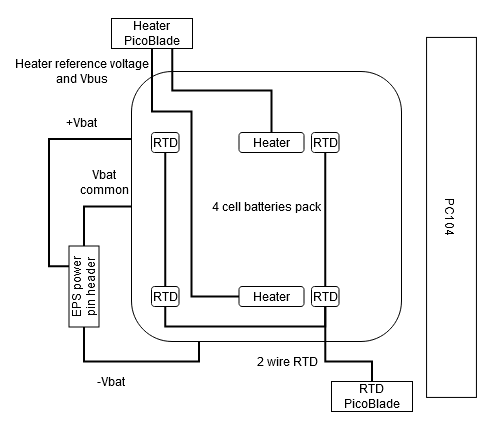
\includegraphics[width=0.65\textwidth]{figures/bat4c_block_diagram}
        \caption{Battery Module 4C Block Diagram.}
        \label{fig:block-diagram}
    \end{center}
\end{figure}
    %
% hardware.tex
%
% Copyright (C) 2021 by SpaceLab.
%
% Battery Module 4C Documentation
%
% This work is licensed under the Creative Commons Attribution-ShareAlike 4.0
% International License. To view a copy of this license,
% visit http://creativecommons.org/licenses/by-sa/4.0/.
%

%
% \brief Hardware chapter.
%
% \author Gabriel Mariano Marcelino <gabriel.mm8@gmail.com>
% \author André Martins Pio de Mattos <andrempmattos@gmail.com>
% \author Yan Castro de Azeredo <yan.ufsceel@gmail.com>
%
% \institution Universidade Federal de Santa Catarina (UFSC)
%
% \version 0.1.1
%
% \date 2020/01/24
%

\chapter{Hardware} \label{ch:hardware}

This chapter describes the hardware of BAT4C in detail. As mentioned beforehand the board is to be used alongside the EPS2 module, both PCBs are complementary forming the full energy power system of a CubeSat.
  
\begin{figure}[!ht]
    \begin{center}
        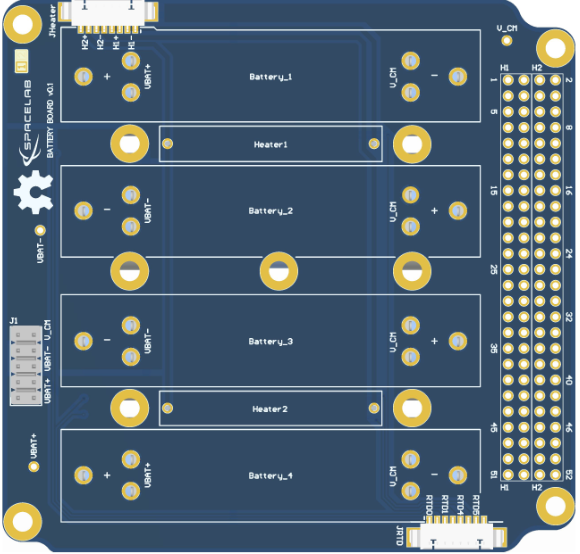
\includegraphics[width=93mm]{figures/bat4c-pcb-top.png}
        \caption{Top side of the PCB.}
        \label{fig:pcb-top}
    \end{center}
\end{figure}

\begin{figure}[!ht]
    \begin{center}
        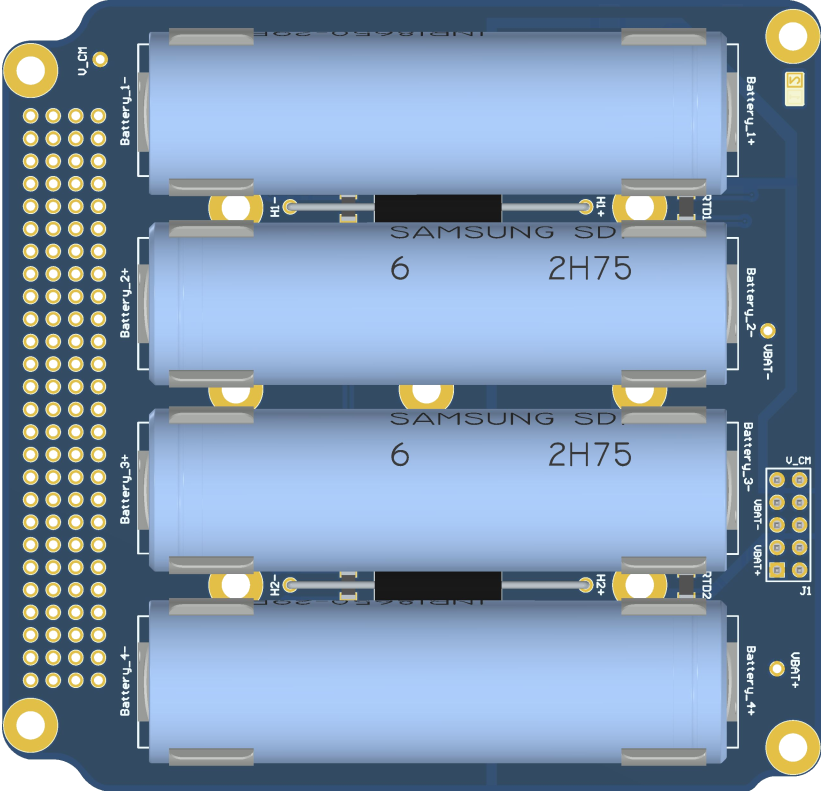
\includegraphics[width=93mm]{figures/bat4c-pcb-bottom.png}
        \caption{Bottom side of the PCB.}
        \label{fig:pcb-bottom}
    \end{center}
\end{figure}

\begin{figure}[!ht]
    \begin{center}
        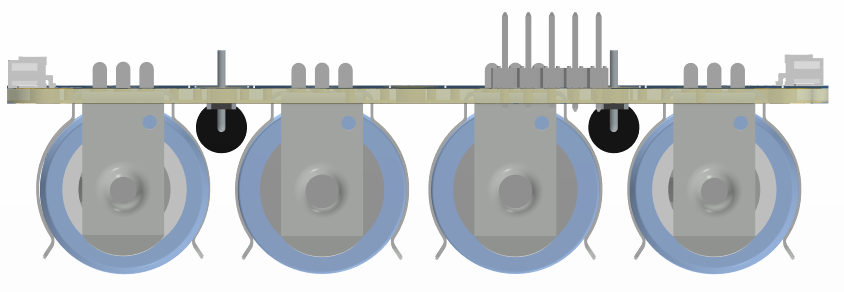
\includegraphics[width=93mm]{figures/bat4c-pcb-front.png}
        \caption{Front side of the PCB.}
        \label{fig:pcb-front}
    \end{center}
\end{figure}


\section{External Connectors}

The external interfaces are connected to the EPS with board to board and cable to cable connectors. The following topics describes these interfaces and present their pinout.

\subsection{JRTD - RTD PicoBlade}

The RTDs on the board are connected to the EPS2 with the labeled "JRTD" 8 pin right angle PicoBlade (\textbf{53261-0871}), its pinout is showed on \autoref{tab:picoblade-rtd}. The connector can be seen in \autoref{fig:rtd-picoblade}.

\begin{table}[!h]
    \centering
    \begin{tabular}{cllll}
        \toprule[1.5pt]
        \textit{Pin} & \textit{Row} \\
        \midrule
        1            & RTD0         \\
        2            & RTD\_Common  \\
        3            & RTD1     \\
        4            & RTD\_Common  \\
        5            & RTD4         \\
        6            & RTD\_Common  \\
        7            & RTD5         \\
        8            & RTD\_Common  \\
        \bottomrule[1.5pt]
    \end{tabular}
    \caption{RTD PicoBlade pinout.}
    \label{tab:picoblade-rtd}
\end{table}

\begin{figure}[!ht]
    \begin{center}
        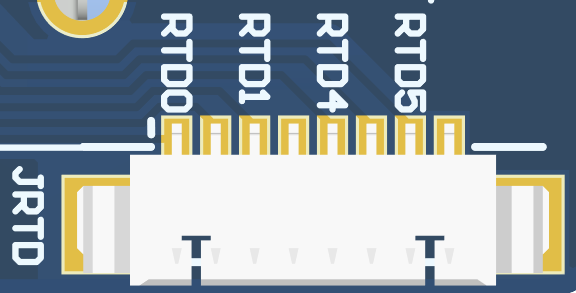
\includegraphics[width=0.35\textwidth]{figures/rtd-picoblade.png}
        \caption{RTD PicoBlade connector.}
        \label{fig:rtd-picoblade}
    \end{center}
\end{figure}

\subsection{JHeater - PicoBlade}

The heaters controled supply is done with another 8 pin right angle PicoBlade labeled "JHeater", its pinout showed on \autoref{tab:heater-picoblade}. The Vbus pins brings the direct power from the main power bus from the EPS2 module, thought PMW it controls mosfets gates closing the circuit allowing current flow across the heaters. The connector can be seen in \autoref{fig:heater-picoblade}.

\begin{table}[!h]
    \centering
    \begin{tabular}{cllll}
        \toprule[1.5pt]
        \textit{Pin} & \textit{Row} \\
        \midrule
        1            & $-$Heater1\_Voltage  \\
        2            & $-$Heater1\_Voltage  \\
        3            & VBus                 \\
        4            & VBus                 \\
        5            & $-$Heater2\_Voltage  \\
        6            & $-$Heater2\_Voltage  \\
        7            & VBus                 \\
        8            & VBus                 \\
        \bottomrule[1.5pt]
    \end{tabular}
    \caption{Heater PicoBlade pinout.}
    \label{tab:heater-picoblade}
\end{table}

\begin{figure}[!ht]
    \begin{center}
        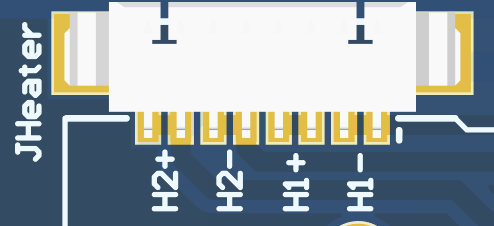
\includegraphics[width=0.35\textwidth]{figures/heater-picoblade.png}
        \caption{Heater PicoBlade connector.}
        \label{fig:heater-picoblade}
    \end{center}
\end{figure}

\subsection{J1 - Battery Voltage Pin Header}

A pin header connector (\textbf{67996-110HLF}) labeled "J1" connects to the EPS2 module in a board to board style. These pins brings the voltage from the 4 cell batteries and a common reference voltage to be used for the battery monitor IC present on the EPS2. Its pinout can be seen on \autoref{tab:battery-pin-header} and connector view on \autoref{fig:battery-pin-header}.

\begin{table}[!h]
    \centering
    \begin{tabular}{cllll}
        \toprule[1.5pt]
        \textit{Pin} & \textit{Row} \\
        \midrule
        1            & $+$Vbat \\
        2            & $+$Vbat \\
        3            & $+$Vbat \\
        4            & $+$Vbat \\
        5            & $-$Vbat \\
        6            & $-$Vbat \\
        7            & $-$Vbat \\
        8            & $-$Vbat \\
        9            & Vbat\_Common \\
        10           & Vbat\_Common \\
        \bottomrule[1.5pt]
    \end{tabular}
    \caption{Battery voltage pin header pinout.}
    \label{tab:battery-pin-header}
\end{table}

\begin{figure}[!ht]
    \begin{center}
        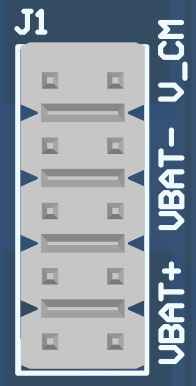
\includegraphics[width=0.2\textwidth]{figures/battery-pin-header.png}
        \caption{Battery pin header connector.}
        \label{fig:battery-pin-header}
    \end{center}
\end{figure}

\subsection{PC104}

On revision v0.1 of the project, the BAT4C does not use the PC104 for any purpose, been mechanical or electrical.

\section{Batteries}

Each 18650 size battery cell is fixed with metal holder (\textbf{54}). The pollarity for each cell is visible on the silkcreen on the board as can be seen in \autoref{fig:pcb-top}. The metal holders are soldered on the though hole pads, the exposed square pads are a simple solution for soldering the cells to the board and keeping them in place during vibrations, see \autoref{fig:battery-pads}. This particular solution might suffer improvements in later hardware releases.

\begin{figure}[!ht]
    \begin{center}
        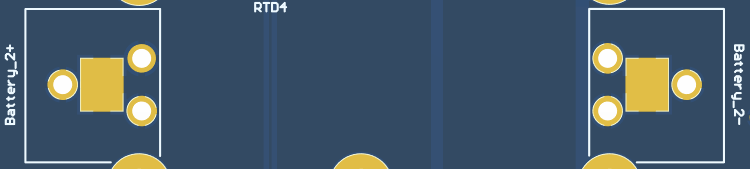
\includegraphics[width=0.75\textwidth]{figures/battery-pads.png}
        \caption{Bottom side of the PCB.}
        \label{fig:battery-pads}
    \end{center}
\end{figure}

\section{Temperature Sensors}

Temperature of the board is measured with four RTDs (\textbf{32207595}), two placed near the batteries contacts and the other two in the middle between the cells and below the heaters legs, as can be seen on \autoref{fig:rtds-heaters-view}. The RTDs are Pt1000 Class B accuracy, its datasheet can be acessed here \cite{rtd-datasheet} for more technical spececification of the sensors.

\begin{figure}[!ht]
    \begin{center}
        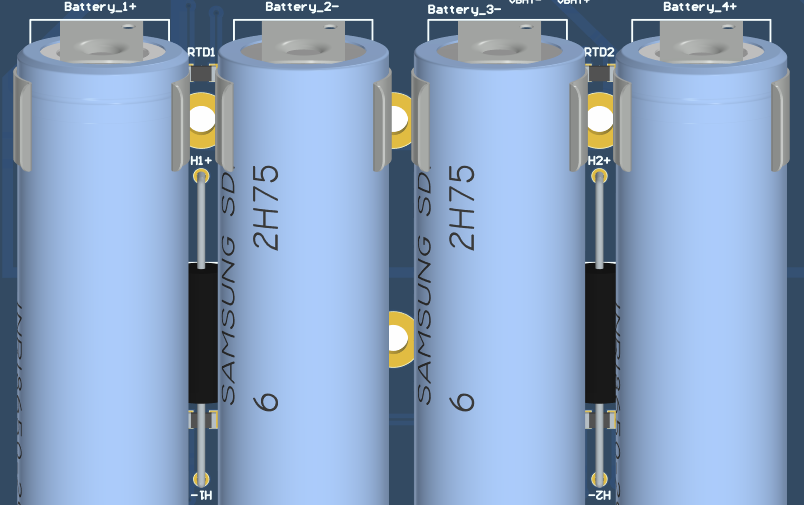
\includegraphics[width=0.75\textwidth]{figures/rtds-heaters-view.png}
        \caption{RTDs and heaters view.}
        \label{fig:rtds-heaters-view}
    \end{center}
\end{figure}

\section{Heaters}

Wirewound resistors (\textbf{RS02B24R00FE12}) are used for the two heaters placed on the board between the cells, as previously seen in \autoref{fig:rtds-heaters-view}. Their purpose is to maintain the cells temperature during eclipse periods, where a CubeSat can reach temperatures below $-$20 degrees celsius. While the resistors can deliver up to a maximum of 3 watts of power, controled PWM signals from the EPS2 regulates this energy dissipation to secure and ideal levels for the cells normal operation.
    %
% references.tex
%
% Copyright (C) 2021 by SpaceLab.
%
% Battery Module 4C Documentation
%
% This work is licensed under the Creative Commons Attribution-ShareAlike 4.0
% International License. To view a copy of this license,
% visit http://creativecommons.org/licenses/by-sa/4.0/.
%

%
% \brief References chapter.
%
% \author Gabriel Mariano Marcelino <gabriel.mm8@gmail.com>
% \author André Martins Pio de Mattos <andrempmattos@gmail.com>
% \author Yan Castro de Azeredo <yan.ufsceel@gmail.com>
%
% \institution Universidade Federal de Santa Catarina (UFSC)
%
% \version 0.1.1
%
% \date 2020/11/07
%

\bibliography{references/eps2, references/battery-board-1, references/bat4c}

\addcontentsline{toc}{chapter}{References}


\end{document}
